% Condition H (Orthogonal + Taxonomy) - Mechanism Hierarchy
\begin{figure}[H]
\centering
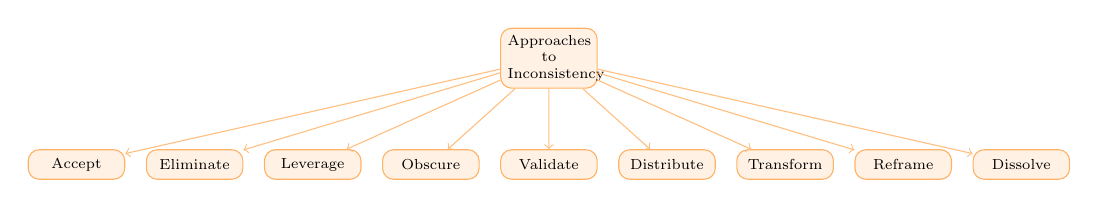
\begin{tikzpicture}[scale=0.75, transform shape,
  grow=south,
  level 1/.style={sibling distance=2.0cm, level distance=1.8cm},
  every node/.style={rectangle, rounded corners, draw=orange!60, fill=orange!10, font=\scriptsize, align=center, text width=1.4cm, minimum height=0.5cm},
  edge from parent/.style={draw, orange!50, ->},
]
\node {Approaches to\\Inconsistency}
  child {node {Accept}}
  child {node {Eliminate}}
  child {node {Leverage}}
  child {node {Obscure}}
  child {node {Validate}}
  child {node {Distribute}}
  child {node {Transform}}
  child {node {Reframe}}
  child {node {Dissolve}}
;
\end{tikzpicture}
\caption{Condition H mechanism-tree schematic. Nine curator-authored stances toward inconsistency are shown beneath a synthetic super-root; solution nodes, candidate-to-mechanism links, and lower mechanism branches are omitted. One additional candidate-text mechanism root retained in the database is not shown, yielding the ten-root total in Table~\ref{tab:graph-stats}.}
\label{fig:tree-h}
\end{figure}
